% fig05 — First-event contribution map for the type-1 backward equation
% Standalone TikZ. Build:  latexmk -pdf fig05.tex   (or pdflatex fig05.tex x2)
% Matches sections/02_model.tex, "First-event calculation".
\documentclass[border=6pt]{standalone}

\usepackage[T1]{fontenc}
\usepackage{lmodern}          % Latin Modern, matching the paper
\usepackage{amsmath,amssymb,mathtools}
\usepackage{multirow}         % dot spanning both header lines
\usepackage{xcolor}
\usepackage{tikz}
\usetikzlibrary{positioning,calc,arrows.meta,shapes.geometric,backgrounds}

% ---- paper macros -----------------------------------------------------------
\newcommand{\dd}{\mathrm d}
\newcommand{\Rstate}{\mathsf R}   % absorbing catastrophe state (R,R)

% ---- palette (SHARED_CONVENTIONS.md) ---------------------------------------
\definecolor{t1blue}{HTML}{0072B2}   % type 1 / S
\definecolor{t2verm}{HTML}{D55E00}   % type 2 / G
\definecolor{ink}{HTML}{1a1c1f}      % near-black
\definecolor{soft}{HTML}{565b62}     % secondary text
\definecolor{gridc}{HTML}{e3e6ea}    % light rules
\definecolor{okgreen}{HTML}{2e7d32}  % certain survival (value 1)
\definecolor{warn}{HTML}{b06a00}
\definecolor{errred}{HTML}{9a2820}   % catastrophe (value 0)
\definecolor{panelbg}{HTML}{fafafa}

% ---- reusable styles --------------------------------------------------------
\tikzset{
  % distribution wiring
  wire/.style={draw=soft, line width=0.9pt, -{Stealth[length=2.1mm,width=1.9mm]}},
  busline/.style={draw=soft, line width=0.9pt},
  % tokens (individuals)
  tok/.style={circle, minimum size=6.4mm, inner sep=0pt, draw=white, line width=0.5pt},
  t1tok/.style={tok, fill=t1blue},
  t2tok/.style={tok, fill=t2verm},
  % catastrophe absorbing marker: stop-sign octagon
  rmark/.style={regular polygon, regular polygon sides=8, fill=errred, draw=errred!60!black,
                line width=0.4pt, text=white, minimum size=8.5mm, inner sep=0pt, font=\bfseries},
  % rate pill on the branch
  pill/.style={rounded corners=2pt, draw=#1, line width=0.8pt, fill=white,
               inner xsep=4pt, inner ysep=2.5pt, font=\normalsize, text=ink},
  % light box around an ODE result
  odebox/.style={rounded corners=3pt, draw=#1!70, line width=1pt, fill=#1!6,
                 inner xsep=9pt, inner ysep=6pt},
}

% Card geometry (type 1, main)
\newcommand{\Whalf}{1.62}      % half card width
\newcommand{\cardTop}{5.55}
\newcommand{\cardBot}{2.08}
\newcommand{\headBot}{4.95}    % bottom of coloured header strip

% One MAIN card. Args:
% #1 centre x  #2 accent colour  #3 header text colour  #4 event name
% #5 token-drawing code (tikz)   #6 reason (short)      #7 contribution (math)
% #8 contribution colour
\newcommand{\maincard}[8]{%
  % body
  \fill[#2!7, rounded corners=4pt] (#1-\Whalf,\cardBot) rectangle (#1+\Whalf,\cardTop);
  % header strip
  \fill[#2, rounded corners=4pt] (#1-\Whalf,\headBot) rectangle (#1+\Whalf,\cardTop);
  \fill[#2] (#1-\Whalf,\headBot) rectangle (#1+\Whalf,{\headBot+0.18}); % square off header bottom
  \draw[#2, line width=1pt, rounded corners=4pt] (#1-\Whalf,\cardBot) rectangle (#1+\Whalf,\cardTop);
  \node[text=#3, font=\bfseries\small] at (#1,{(\headBot+\cardTop)/2}) {#4};
  % tokens
  \begin{scope}[shift={(#1,4.18)}] #5 \end{scope}
  % reason
  \node[text=soft, font=\scriptsize, align=center, text width=3.0cm] at (#1,3.42) {#6};
  % separator + value
  \draw[gridc, line width=0.8pt] (#1-\Whalf+0.18,3.02) -- (#1+\Whalf-0.18,3.02);
  \node[text=soft, font=\scriptsize] at (#1,2.78) {contributes};
  \node[text=#8, font=\large] at (#1,2.43) {$#7$};
}

\begin{document}
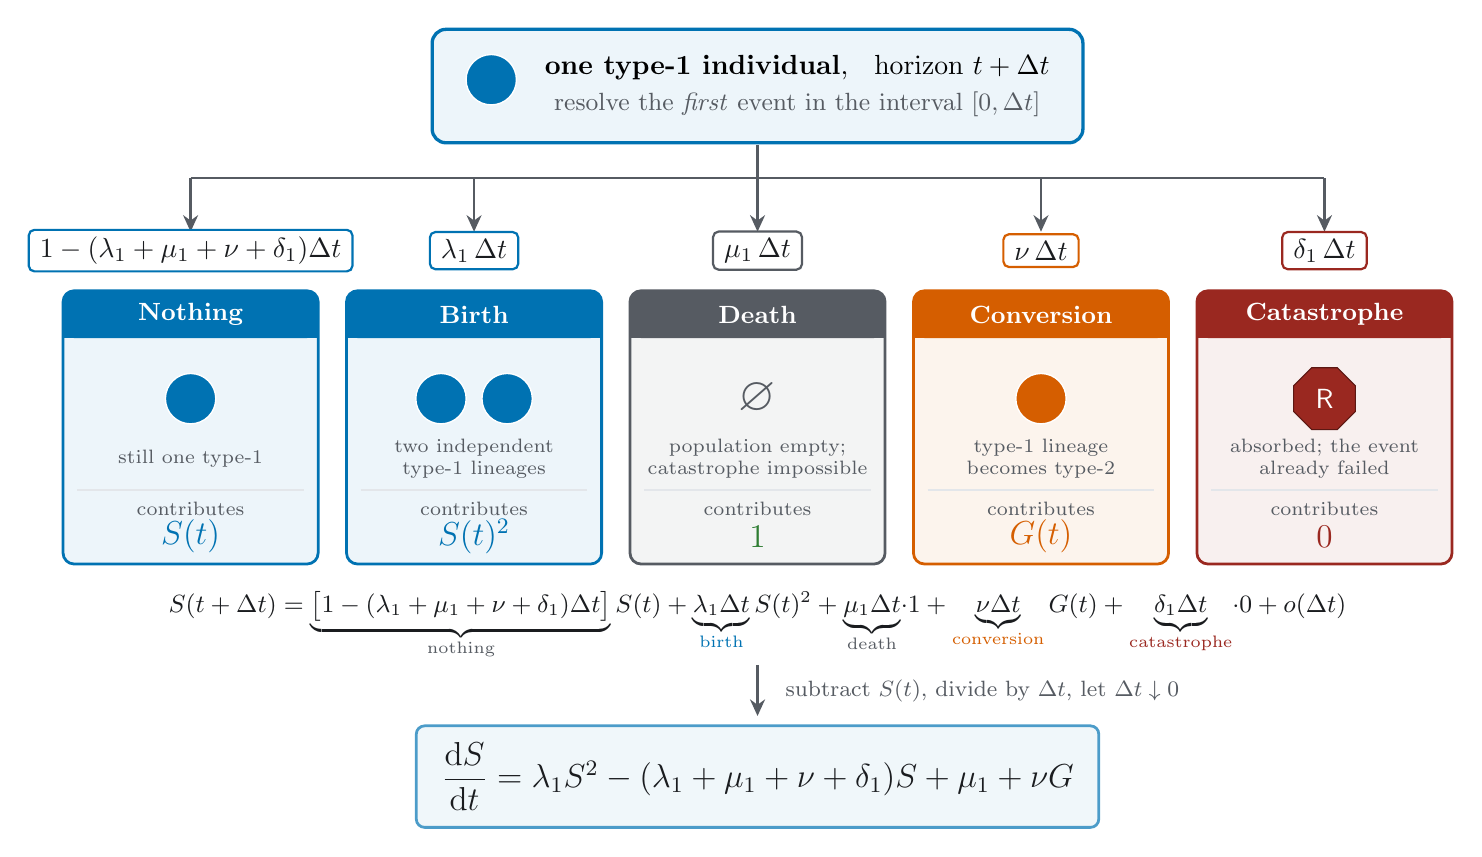
\begin{tikzpicture}[
    every node/.style={inner sep=0pt},
    x=1cm, y=1cm,
]

% =====================================================================
%  TYPE 1  (main)
% =====================================================================
\def\XA{0} \def\XB{3.6} \def\XC{7.2} \def\XD{10.8} \def\XE{14.4}

% ---- source state ---------------------------------------------------
\node[rounded corners=5pt, draw=t1blue, line width=1.2pt, fill=t1blue!7,
      inner xsep=12pt, inner ysep=8pt] (src) at (\XC,8.15)
     {\begin{tabular}{@{}c@{\ \ \ }c@{}}
        \multirow{2}{*}{\tikz\node[t1tok]{};} &
          \textbf{one type-1 individual}, \; horizon $t+\Delta t$\\[1pt]
        & {\small\color{soft} resolve the \emph{first} event in the interval $[0,\Delta t]$}
      \end{tabular}};

% ---- distribution bus ----------------------------------------------
\def\busY{6.98}
\draw[busline] (\XC,7.40) -- (\XC,\busY);
\draw[busline] (\XA,\busY) -- (\XE,\busY);
\foreach \x in {\XA,\XB,\XC,\XD,\XE}{ \draw[wire] (\x,\busY) -- (\x,6.30); }

% ---- rate pills (probability of that event in Delta t) -------------
\node[pill=t1blue]  at (\XA,6.06) {$1-(\lambda_1+\mu_1+\nu+\delta_1)\Delta t$};
\node[pill=t1blue]  at (\XB,6.06) {$\lambda_1\,\Delta t$};
\node[pill=soft]    at (\XC,6.06) {$\mu_1\,\Delta t$};
\node[pill=t2verm]  at (\XD,6.06) {$\nu\,\Delta t$};
\node[pill=errred]  at (\XE,6.06) {$\delta_1\,\Delta t$};

% ---- five cards -----------------------------------------------------
\maincard{\XA}{t1blue}{white}{Nothing}
  {\node[t1tok]{};}
  {still one type-1}{S(t)}{t1blue}

\maincard{\XB}{t1blue}{white}{Birth}
  {\node[t1tok] at (-0.42,0){}; \node[t1tok] at (0.42,0){};}
  {two independent type-1 lineages}{S(t)^2}{t1blue}

\maincard{\XC}{soft}{white}{Death}
  {\node[font=\LARGE,text=soft] {$\varnothing$};}
  {population empty; catastrophe impossible}{1}{okgreen}

\maincard{\XD}{t2verm}{white}{Conversion}
  {\node[t2tok]{};}
  {type-1 lineage becomes type-2}{G(t)}{t2verm}

\maincard{\XE}{errred}{white}{Catastrophe}
  {\node[rmark]{$\Rstate$};}
  {absorbed; the event already failed}{0}{errred}

% ---- assembly line --------------------------------------------------
\node[font=\small, text=ink] (asm) at (\XC,1.30) {$
  S(t+\Delta t)=
  \underbrace{\bigl[1-(\lambda_1+\mu_1+\nu+\delta_1)\Delta t\bigr]}_{\text{\color{soft}nothing}}S(t)
  +\underbrace{\lambda_1\Delta t}_{\text{\color{t1blue}birth}}S(t)^2
  +\underbrace{\mu_1\Delta t}_{\text{\color{soft}death}}\!\cdot 1
  +\underbrace{\nu\Delta t}_{\text{\color{t2verm}conversion}}G(t)
  +\underbrace{\delta_1\Delta t}_{\text{\color{errred}catastrophe}}\!\cdot 0
  +o(\Delta t)
$};

% ---- limit arrow + ODE ---------------------------------------------
\draw[wire, line width=1pt] (\XC,0.80) -- (\XC,0.15);
\node[text=soft, font=\footnotesize, anchor=west] at (\XC+0.35,0.47)
     {subtract $S(t)$, divide by $\Delta t$, let $\Delta t\downarrow 0$};
\node[odebox=t1blue, font=\large, text=ink] at (\XC,-0.62)
     {$\dfrac{\dd S}{\dd t}=\lambda_1 S^2-(\lambda_1+\mu_1+\nu+\delta_1)S+\mu_1+\nu G$};

\end{tikzpicture}
\end{document}
